\documentclass[aps, twocolumn, groupedaddress]{revtex4}
%preprint,
%\documentclass[10pt]{report}  
\usepackage[xdvi]{graphics}
\usepackage{graphicx}
\usepackage{pdfsync}
\def\al{\alpha}
%\def\k{\k}
\def\w{p}
\def\pc{\pi}
%\def\t{\t}
\def\T{S}
%\def\e{\e}
%\def\p{\p}
\def\R{w_{r}}
\def\a{\rho}
\def\n{\n}
\def\g{Q}
\def\s{t_0}
\def\J{j}
\def\I{n}
\def\t{t}
\def\zt{{\tilde Z}}
\def\ord{{\cal O}}
\def\AB{BA\ }

\newcommand{\lb}{{\langle}}
\newcommand{\rb}{{\rangle}}
\newcommand{\rv}{\textbf{r}}
\newcommand{\rW}{\textbf{W}}

\begin{document}

\title{The Diameter and Chemical Distance of Random Clusters}

\author{Don Blair}
\author{Jon Machta}
\affiliation{Department of Physics, University of Massachusetts, Amherst, MA 01003-3720}
\begin{abstract}

We report numerical results for the fractal dimension of the diameter (the ``longest shortest path'' between vertices along bonds) and the chemical distance of 2D and 3D Potts clusters for $q=1,2,3,4$.  We find that the fractal dimension of the diameter and of the chemical distance of Potts clusters are equal to within numerical error, and we suggest a possible relationship between $D_{min}$ and the dynamical exponent, $z$.

\end{abstract}

\maketitle

\section{Background}

%%%POTTS MODEL AND APPLICATIONS%%%

The Potts Model, initially introduced as a generalization of the 2-state Ising Model to $q$ possible spin states, can in fact be mapped onto the Random Cluster Model for all $q \ge 0$, with $q \to 1$ corresponding to the Percolation Model, and $q \to 2$ corresponding to the Ising Model.  The Potts Model has found application in an impressively diverse range of applications, including conformal field theory, percolation theory, knot theory, quantum groups, mathematical biology, and complex networks.
%more specific ...
Although easy to formulate, the model exhibits rich phase behavior, and its study has yielded many significant insights into critical phenomena in statistical physics. 

An important geometric property of Potts clusters that has proved very useful in describing transport and diffusion processes in random media is the ``chemical distance'', $l$ -- the length of the ``chemical'' or shortest path between two randomly chosen sites on a cluster.  The average chemical distance on critical Potts clusters has been shown to scale as $\bar{l} \propto r^{d_{min}}$ at criticality, where $r$ is the Euclidean distance between the endpoints of the chemical path $l$. Attempts to establish a relationship between $d_{min}$ and other known critical exponents have, as yet, proved inconclusive [refs].  For the $q \to 1$ (Percolation) case, much work has already been done to determine $d_{min}$ numerically \cite{Gr83, HrSt88} and an exact solution has been found using results from conformal field theory \cite{Zi99}.
 
In this paper we generalize previous studies of $d_{min}$ for the 2D, $q=1$ Potts Model by reporting results for the $q = 2, 3$ and $4$ for both Potts Models in both 2D and 3D.  We also study the critical scaling of a related quantity: the diameter, $D$, defined as the longest of all the shortest paths between points on a cluster. (An illustration of both $D$ and $l$ on a Potts cluster is shown in Figure [A]).  We show that $D$ also exhibits scaling behavior at criticality: $\bar{D} \propto r^{D_{min}}$; and that, significantly, $d_{min} = D_{min}$ to within the error of our numerical results.  
 
We also propose a possible relationship between both $D_{min}$ $d_{min}$ and the dynamical exponent, $z$.

%%%TWO PEAKS IN HISTOGRAM%%%
%The histogram for $q>2$ seems to exhibit two peaks.

\section{Methods}

\subsection{Potts Model Simulation}
--Swedsen Wang.

--Random Number Generator.

--Correlation time.

--Time to reach equilibrium.

--Bootstrap method as check

\subsection{Determining the chemical distance and the diameter}
--Chemical distance.

--Naive method for diameter.

--Our method for the diameter.

%\begin{figure}[ht]
%\begin{center}
%\scalebox{.7}{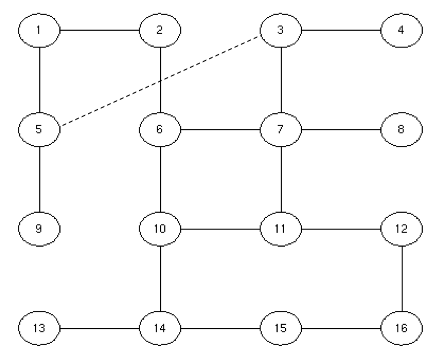
\includegraphics{nodes}}
%\caption{\label{fig:nodes} $\phi = 0.05$. 2000 particle simulation. Times shown (indicated in brackets above each sample) are 0, 300, 600, and 42000 GROMACS times units. The last time shown is the last time available in the simulation (running speed is $\phi$-dependent.}
%\end{center}
%\end{figure}

\section{Results and Discussion}

%%%DATA FOR dmin 2D%%%
\subsection{Results for 2D Potts Model}

-- Correlation time and time to reach equilibrium.

-- Correspondence bewteen $d_{min}$ and $D_{min}$ for $L \le 128$.

-- Results for $d_{min}$ for $L > 128$.

\begin{table}[h]
\begin{center}
\begin{tabular}{| l | l | l | l | l | l | l |}
\hline
$q$ & 1 & 2 & 3 & 4 \\
\hline
$d_{min}$ & 1.127(3) & 1.0911(2) & 1.060(1) & 1.023(7) \\
\hline
$D_{min}$ & 1.129(2) & 1.09(1) & 1.059(2) & 1.025(2) \\
\hline
\end{tabular}
\caption{\label{tab:dminD} {\bf Results for 2D Potts Model.} Scaling exponent for the chemical distance ($d_{min}$) and for the diameter ($D_{min}$) for the 2D Potts model with various values of $q$, with system size L=4, 8, 16, 32, 48, 64, 96, 128.}
\end{center}
\end{table}


\subsection{Results for 3D Potts Model}

-- Correlation time and time to reach equilibrium.

-- Correspondence between $d_{min}$ and $D_{min}$ for $L \le 96$.

-- Results for $d_{min}$ for $L > 96$.

\begin{table}[h]
\begin{center}
\begin{tabular}{| l | l | l | l | l | l | l |}
\hline
$q$ & 1 & 2 & 3 & 4 \\
\hline
$d_{min}$ & 1.127(3) & 1.0911(2) & 1.060(1) & 1.023(7) \\
\hline
$D_{min}$ & 1.129(2) & 1.09(1) & 1.059(2) & 1.025(2) \\
\hline
\end{tabular}
\caption{\label{tab:dminD} {\bf Results for 3D Potts Model.} Scaling exponent for the chemical distance ($d_{min}$) and for the diameter ($D_{min}$) for the 3D Potts model with various values of $q$, with system size L=4, 8, 16, 32, 48, 64, 96, 128.}
\end{center}
\end{table}

\subsection{Postulated Relationship between $D_{min}$ and $z$}

Diffusion exponent, dynamic exponent, argument for relationship.


\acknowledgements
This work was supported by NSF grant ()
\bibliographystyle{apsrev}
%\bibliographystyle{unsrt}
\bibliography{../bibfiles/dwbreferences}
  

\end{document}
